\documentclass[12pt,UTF8]{ctexbook}
\usepackage{ctex}
\usepackage{array}
\usepackage{graphicx}
\usepackage{wrapfig}
\usepackage[table,dvipsnames]{xcolor}
\usepackage{tabularx}
\usepackage{amsmath}
\usepackage{amssymb}
\usepackage{xfrac}
\usepackage{eucal}
\usepackage{titlesec}
\usepackage{amsthm}
\usepackage{tikz-cd}
\usepackage{enumitem}
\usepackage{verbatim}
\usepackage{fontspec,xunicode,xltxtra}
\usepackage{xeCJK} 
\usepackage{caption}

\definecolor{gl}{RGB}{246, 252, 240}
\definecolor{gd}{RGB}{236, 244, 230}
\definecolor{bg}{RGB}{242, 244, 228}


\setCJKmainfont[BoldFont=STZhongsong]{STSong}
\setCJKmonofont{simkai.ttf} % for \texttt
\setCJKsansfont{simfang.ttf} % for \textsf
\setlength\parskip{8pt}
\setlength{\fboxsep}{12pt}
\renewcommand\thesection{\arabic{chapter}.\arabic{section}}
\newtheorem{df}{定义}[section] 
\newtheorem{pp}{命题}[section]
\newtheorem{tm}{定理}[section]
\newtheorem{ex}{例子}[section]
\newtheorem{et}{例题}[section]
\newtheorem{sk}{思考}[section]
\newtheorem*{so}{解答}
\newenvironment{proof2}{\paragraph{\textbf{证明:}}}{\hfill$\square$}
\newtheorem{xt}{习题}[section]
\newtheorem{cor}{推论}[pp]
% 列举环境的行间距
\setenumerate[1]{itemsep=0pt,partopsep=0pt,parsep=0pt,topsep=0pt}
\setitemize[1]{itemsep=0pt,partopsep=0pt,parsep=0pt,topsep=0pt}
\setdescription{itemsep=0pt,partopsep=0pt,parsep=0pt,topsep=0pt}
% 章节字体大小
\titleformat{\section}{\zihao{-2}\bfseries}{ \thesection }{16pt}{}
% 封面
\title{\zihao{0} \bfseries 第一册}
\author{\zihao{2} \texttt{大青花鱼}}
% \date{\bfseries\today}
\date{}
% 正文
\begin{document}
\maketitle
\tableofcontents
\newpage

\chapter{数列初步}

\section{数列的基本概念}

\begin{ex}
    \mbox{}\\
\indent 1. 把自然数的倒数排成一列:
$$ 1,\,\,\, \frac{1}{2}, \,\,\, \frac{1}{3}, \,\,\,\frac{1}{4}, \,\,\,\frac{1}{5}, \cdots $$

2. 把圆周率按个位,十分位、百分位、千分位截断,得到一列数:
$$  3,\,\,\, 3.1,\,\,\, 3.14,\,\,\, 3.141,\,\,\, 3.1415, \cdots   $$

    3. 把班上同学的身高(厘米)按学号排列:
$$ 165,\,\,\, 173,\,\,\, 169,\,\,\, 178, \,\,\,171.5,\,\,\, 176, \cdots  $$
\end{ex}
把数按照一定顺序排列起来,叫做\textbf{数列}。数列中的每一个数叫做数列的一\textbf{项}。
按照顺序,各项分别称为数列的第$1$项、第$2$项,等等。
比如,例$1$中的数列第$2$项是$\frac{1}{2}$,例$2$中的数列第$3$项是$3.14$。

数列的项和序数有一一对应的关系,这告诉我们,数列的本质是正整数集或其子集$[1\ldots N]$到数域的函数。
定义域是$[1\ldots N]$的数列,项数有限,称为\textbf{有穷数列};定义域是正整数集的数列,项数无限,叫做\textbf{无穷数列}。
我们一般把数列记作:
$$ a_1, a_2, \cdots, a_n, \cdots $$
其中$a_n$是数列的第$n$项。项数$n$也叫做\textbf{下标}。
为了方便,我们在行文中会把以上数列记作$\{a_n\}_{n\in\mathbb{Z}^+}$(无穷数列)
或$\{a_n\}_{n\in[1\ldots N]}$(有穷数列),或简单记作$\{a_n\}$。
比如,例$1$中的数列可以记为$\left\{\frac{1}{n}\right\}_{n\in\mathbb{Z}^+}$。
作为函数,如果某数列的序数和项之间的对应关系可以用一个公式来表示,
我们就把这个公式称为该数列的\textbf{通项公式}。比如,例$1$中的数列,通项公式是$a_n = \frac{1}{n}$;
而例$3$中的数列,我们不知道通项公式。有通项公式的数列,只要把序数代入公式,就能得到该项的值。
比如,例$1$中的数列,第$100$项是$\frac{1}{100}$。

我们把各项不断增大(减小)的数列称为\textbf{单调递增(递减)数列}。“单调”一词,表示数列各项增减方向保持一致。
换句话说,如果数列$\{a_n\}_{n\in\mathbb{Z}^+}$从第二项起,总有$a_{n+1} \geqslant a_n$,
就说它是\textbf{单调递增数列};如果总有总有$a_{n+1} \leqslant a_n$,就说它是\textbf{单调递减数列}。如果要求不能有相等的项,
就称为\textbf{严格单调递增(递减)数列}。

研究数列的一个基本目的,是对数列进行求和。比如,一垛炮弹有$8$层,顶层有$1$个炮弹,第$2$层有$4$个,
第$3$层有$9$个,……,第$8$层有$64$个,我们希望知道一共有几个炮弹。把各层炮弹个数记为数列:$a_1 = 1$
$$ a_1 = 1, a_2 = 4, \cdots, a_8 = 64 $$
我们把数列的和记为$S_8 = a_1 + a_2 + \cdots + a_8$。为了方便,我们也用求和符号表示数列的和:$S_8 = \sum_{i=1}^8 a_i$。对于无穷数列,我们还无法定义数列的和,只能定义它的部分和:$S_N = \sum_{i=1}^N a_i$。我们把$S_N$称为数列$\{a_n\}$的前$N$项和。比如,例$1$中的数列的前$4$项和为:
$$ S_4 = 1 + \frac{1}{2} + \frac{1}{3} + \frac{1}{4} =  \frac{25}{12}. $$

\begin{xt}
    \mbox{}\\
\indent 1. 根据以下数列的通项公式,写出数列的前$5$项:\\
\indent 1.1. $a_n = n^2$ \\
\indent 1.2. $a_n = (-1)^n \cdot n$ \\
\indent 1.3. $a_n = \frac{n}{n+3}$ \\
\indent 1.4. $a_n = 2^n - 1$ \\
\indent 1.5. $a_n = \frac{(-2)^n + n - 1}{n^2 + 1}$ \\
\indent 2.根据以下数列的通项公式,计算数列的前$5$项和与前$7$项和: \\
\indent 2.1. $a_n = n^2$ \\
\indent 2.2. $a_n = (-1)^{n+1} \cdot n$ \\
\indent 2.3. $a_n = \frac{2}{n(n+1)}$ \\
\indent 2.4. $a_n = 2^n$ \\
\indent 2.5. $a_n = (n+1)2^{n}$ \\
\indent 3. 已知数列$\{a_n\}_{n\in\mathbb{Z}^+}$,如何构造一个数列$\{b_n\}_{n\in\mathbb{Z}^+}$,
使得它的前$n$项和是$a_n$?
\end{xt}

无穷数列(或项数相同的有穷数列)作为函数,可以进行函数之间的四则运算。
比如,设无穷数列$\{a_n\}$和$\{b_n\}$的通项公式分别是$a_n = n - 1$、$b_n = 2n$,
那么对任意正整数$n$,$a_n + b_n = 3n - 1$。
我们定义通项公式为$c_n = 3n - 1$的数列$\{c_n\}$为$\{a_n\}$与$\{b_n\}$的和,也就是说,
我们定义数列的加法:$\{a_n\} + \{b_n\} = \{a_n + b_n\}$。

可以验证,数列的加法满足交换律和结合律。我们称每项都等于同一个数的数列为\textbf{常数列},
任何数列加上常数列$\{0\}$都等于自己。

同理,我们可以定义数列的减法和乘法。它们满足的运算律和有理数的运算律一致。
任何数列乘以$\{1\}$都得到自己。如果我们把所有取值为实数的数列的集合记为$\mathbb{R}^\mathbb{N}$,
那么$\mathbb{R}^\mathbb{N}$和$\mathbb{Z}$一样,可以“装载”加法、减法和乘法。
其中的常数列$\{0\}$、$\{1\}$就相当于整数$0$和$1$。

此外,给定数列$\{a_n\}$和实数$t$,我们可以把$\{a_n\}$的每一项乘以$t$得到一个新数列:
$t\cdot \{a_n\} = \{t\cdot a_n\}$,这个运算称为\textbf{数乘运算}。数乘运算和数、数列的四则运算相容。
\begin{align}
    \forall  \,\, s, t \in \mathbb{R}, \,\,\, \forall \,\, \{a_n\}, \,\,\,& s \cdot (t\cdot \{a_n\}) = (s\cdot t)\cdot \{a_n\}, \notag \\
    & (s + t) \cdot \{a_n\} = (s\cdot \{a_n\}) + (t\cdot \{a_n\}). \notag \\
    \forall  \,\, t \in \mathbb{R}, \,\,\, \forall \,\, \{a_n\}, \,\, \{b_n\},\,\,\, & t \cdot (\{a_n\} + \{b_n\}) = (t \cdot \{a_n\}) + (t \cdot \{b_n\}). \notag 
\end{align}

无穷数列还可以进行函数操作,与函数复合。比如,我们定义函数$f:\,\,x\mapsto x^2 - 3$,
数列$\{a_n\}$的每一项经过$f$映射到$f(a_n) = f(n-1) = (n-1)^2 - 3 = n^2 - 2n - 2$。
那么数列$\{n^2-2n-2\}$就可以称为$\{a_n\}$经过$f$的\textbf{像数列}。
换句话说,我们用实值函数$f$定义了一个$\mathbb{R}^\mathbb{N}$到$\mathbb{R}^\mathbb{N}$的映射。

另一种对数列的操作方法是通过下标。设$g$是从正整数集映射到正整数集的函数,
比如$g:\,\, n \mapsto 3n - 2$。从$\{a_n\}$出发,考虑数列$\{u_n\}$:$u_n = a_{g(n)} = a_{3n-2}$。
这样定义的$\{u_n\}$称为用$g$从$\{a_n\}$中提取的数列。要注意的是,$g$不一定把$\{a_n\}$中每项恰好提取一次,比如
$$ a_1, a_1, a_2, a_2, a_3, a_3, a_4, a_4, \cdots $$
这样的数列也是从$\{a_n\}$中提取的。如果对任何正整数$n$,函数$g$满足$g(n+1) > g(n)$,
用$g$从$\{a_n\}$中提取的数列就可以看作是从前到后挑出一部分项得到的。这样的数列称为$\{a_n\}$的\textbf{子列}。

\begin{sk}
    \mbox{}\\
\indent 1. 给定数列$\{a_n\}$,它的前$n$项和可以构成一个数列$\{S_n\}$,如何用$\{S_n\}$中的项表示$a_n$?
记$v_n$为$\{a_n\}$前$n$项乘积,能否用数列$\{v_n\}$中的项表示$a_n$?\\
\indent 2. 记平面向量的集合为$\mathbb{V}$,
所有从$\mathbb{R}^\mathbb{N}$到$\mathbb{R}^\mathbb{N}$的映射的集合为$\mathfrak{F}(\mathbb{R}^\mathbb{N})$。
$\mathfrak{F}(\mathbb{R}^\mathbb{N})$和$\mathbb{V}$、$\mathbb{Z}$有什么共同点?有什么不同点?\\
\indent 3. 记所有从正整数集到正整数集的函数的集合为$\mathfrak{F}(\mathbb{Z}^+)$,
数列$\{a_n\}$经过$\mathfrak{F}(\mathbb{Z}^+)$中某个函数$g$可以提取出数列$\{b_n\}$。
$g$满足什么条件时,可以找到另一个$\mathfrak{F}(\mathbb{Z}^+)$中的函数$h$,
用$h$可以从$\{b_n\}$中提取出$\{a_n\}$?
\end{sk}

\begin{xt}
    \mbox{}\\
\indent 1. 计算:$\{6n-1\} - \{3k^2 - k + 2\} \cdot \{2^m+1\}$ 。\\
\indent 2. 已知定义在全体实数上的函数$f:\,\, x\mapsto 2x^2 - x - 4$,
数列$\{a_n\}$的通项公式为$a_n = n + \frac{1}{n}$,计算$\{f(a_n)\}$。\\
\indent 3. 另有定义在全体实数上的函数$g:\,\, x\mapsto 1 - \frac{1}{x}$,计算$\{(f - g)(a_n)\}$。
\end{xt}

研究实际问题的时候,我们可能不会直接得到数列的通项公式,而是各项之间的关系。来看以下的例子:
\begin{et}
培养一种乳酸菌,初始从$3$个单位起培养。每过一定时间,等乳酸菌数量翻倍后,
取出$1$个单位的样本做化验观察,其余继续培养。问每次取出化验后,乳酸菌的数量是几个单位?
\end{et}
\begin{so}
设初始数量为$a_0$,第$n$次取出化验后乳酸菌数量为$a_n$个单位。则数列$\{a_n\}$中的项满足以下的关系:
$$ \forall n \in \mathbb{N}, \quad a_{n+1} = 2a_n - 1. $$
\end{so}
这样的关系称为数列的\textbf{递推关}系,相关公式称为\textbf{递推公式}。
以上公式中,已知$a_0$的值,就能推出$a_1$,继而次第推出$a_2$、$a_3$,等等。
$a_0 = 3$,所以$a_1 = 2\cdot 3 - 1= 5$,$a_2 = 2\cdot 5 - 1= 9$,$a_3 = 2\cdot 9 - 1= 17$……

根据递推关系,已知$a_1$,想要算出$a_{100}$,就必须依次算出$a_2,a_3,\cdots,a_{99}$。
很多时候,我们希望从各项之间的关系,推出通项公式,以更方便地了解数列的性质。

如何从递推关系得出通项公式呢?并没有简便的统一方法。
常见的做法是将递推关系转化为一些已知通项公式的数列的递推关系,再反推出原数列的通项公式。
我们在后面会详细介绍。

\begin{xt}
\mbox{}\\
已知数列的递推公式如下,求数列的前$7$项:\\
\indent 1. $a_1 = 1$,$\forall n \geqslant 1, \,\,\, a_{n+1} = 1 - 2a_n.$\\
\indent 2. $a_1 = 1$,$\forall n \geqslant 1, \,\,\, a_{n+1} = 1 + \frac{1}{a_n - 1}.$\\
\indent 3. $a_1 = 1, \,\, \, a_2 = 3$,$\forall n \geqslant 1, \,\,\, a_{n+2} = 4 + a_n - a_n^2.$\\
\indent 4. $a_1 = 1, \,\, \, a_2 = 1$,$\forall n \geqslant 1, \,\,\, a_{n+2} = a_n +a_{n+1}.$\\
\indent 5. $a_1 = 1, \,\, \, a_2 = 3$,$\forall n \geqslant 1, \,\,\, a_{n+2} = a_n(4 - a_{n+1}).$
\end{xt}

\section{等差数列}
来看这样一个数列:
$$ 1,\,\,3,\,\,5,\,\,7,\,\,9,\,\,11,\,\, 13. $$
这个数列有一个特点:从第二项起,每一项减去前一项的差总是$2$。

一般地,如果某个数列从第二项起,每一项减去前一项的差是同一个常数,
就说这个数列是\textbf{等差数列}。这个常数叫做等差数列的\textbf{公差},通常用字母$d$表示。
比如,数列$2,5,8,11,14$的公差是$3$,$19,15,11,7,3,-1$的公差是$-4$。

如果数列$\{a_n\}$的公差是$d$,那么:
\begin{align}
a_2 &= a_1 + d \notag \\
a_3 &= a_2 + d = a_1 + 2d \notag \\
a_4 &= a_3 + d = a_1 + 3d \notag \\
&\quad \vdots \notag \\
a_n &= a_1 + (n-1)d \notag 
\end{align}
等差数列的通项公式是:$a_n = a_1 + (n-1)d$。
\begin{et}
已知无穷等差数列$1,\,\,8,\,\,15, \cdots$,求它的第$30$项。
\end{et}
\begin{so}
等差数列第一项是$1$,公差是$8-1=7$,所以通项公式是$a_n = 1 + (n-1)\cdot 7 = 7n - 6$。第$30$项$a_{30} = 7\cdot 30 - 6 = 204$。
\end{so}
\begin{et}
已知$\{a_n\}_{n\in\mathbb{N}}$是等差数列,$a_1 = 4$, $a_3 = 9$ ,问$94$是否在数列中?如果是的话,是第几项?
\end{et}
\begin{so}
设公差为$d$,则$a_3 = a_1 + 2d$。代入$a_1$、$a_3$的值,解得$d = 2.5$。于是通项公式为$a_n = 4 + (n-1)\cdot 2.5 = 2.5n + 1.5$。如果有$a_n = 94$,即$2.5n + 1.5=94$,解得$n = 37$。因此$94$在数列中,是第$37$项。
\end{so}

设等差数列$\{a_n\}$的前$n$项和为$S_n$。能否方便地表示$S_n$呢?我们可以这样思考:
\begin{align}
a_{1} + a_{n} &= a_1 + a_1 + (n-1)d = 2a_1 + (n-1)d \notag \\
a_{2} + a_{n-1} &= a_1 + d + a_n - d = a_1 + a_n = 2a_1 + (n-1)d \notag \\
&\vdots \notag \\
a_{n-1} + a_{2} &= a_1 + (n-2)d + a_n - (n-2)d = a_1 + a_n =  2a_1 + (n-1)d \notag \\
a_{n} + a_{1} &= a_1 + a_n = 2a_1 + (n-1)d \notag 
\end{align}
把以上$n$个等式分边相加,就得到:
$$ S_n + S_n = n(a_1 + a_n) = 2na_1 + n(n-1)d. $$
也就是说,前$n$项和$S_n$可以写成
$$ S_n = \frac{n(a_1 + a_n)}{2} = na_1 + \frac{n(n-1)}{2}d. $$
这样我们可以方便地计算等差数列的前$n$项和。比如,求前$n$个自然数的和:$a_n = n-1 = 0 + (n-1)\cdot 1$,
所以$S_n = 0 + \frac{n(n-1)}{2}\cdot 1 = \frac{n(n-1)}{2}$。

\begin{xt}
    \mbox{} \\
    \indent 1. 在$8$和$36$之间插入$6$个数,使得这$8$个数成等差数列。\\
    \indent 2. 设数列$\{a_n\}_{n\in\mathbb{Z}^+}$为等差数列,证明$a_{n+2} + a_n = 2a_{n+1}$。\\
    \indent 3. 等差数列$\{a_n\}_{n\in\mathbb{Z}^+}$中,$a_1 = 0.3$,$a_n = 85.5$,$d = 0.6$,求$n$和$S_n$。\\
    \indent 4. 求前$n$个奇数$1,3,5,\cdots, 2n-1$的和。\\
    \indent 5. 直角三角形的三边成等差数列,求三边比例。\\
    \indent 6. 等差数列$\{a_n\}_{n\in\mathbb{Z}^+}$满足$a_1 = 1$,$a_{10}=43.3$,求$S_{20}$ 。    
\end{xt}

\section{等比数列}

来看这样一个数列:
$$ 1,\,\,2,\,\,4,\,\,8,\,\,16,\,\,32,\,\,64. $$
这个数列有一个特点:从第二项起,每一项除以前一项的商总是$2$。

一般地,如果某个数列从第二项起,每一项与前一项的比值是同一个常数,
就说这个数列是\textbf{等比数列}。这个常数叫做等比数列的\textbf{公比},通常用字母$q$表示。
比如,数列$2,6,18,54,162$的公比是$3$,$192,-48,12,-3,0.75$的公比是$-0.25$。

如果数列$\{a_n\}$的公比是$q$,那么:
\begin{align}
a_2 &= a_1 q  \notag \\
a_3 &= a_2 q = a_1 q^2 \notag \\
a_4 &= a_3 q = a_1 q^3 \notag \\
&\quad \vdots \notag \\
a_n &= a_1 q^{n-1} \notag 
\end{align}
等比数列的通项公式是:$a_n = a_1 q^{n-1}$。
\begin{et}
    已知无穷等比数列$1.2, \,\,1.8,\,\,2.7, \cdots$,求它的第$30$项。    
\end{et}
\begin{so}
等比数列第一项是$1$,公比是$1.8\div1.2=1.5$,所以通项公式是
$$a_n = 1.2 \cdot 1.5^{n-1} = \frac{6\cdot3^{n-1}}{5\cdot2^{n-1}} = \frac{3^n}{5\cdot 2^{n-2}}.$$
第$30$项$a_{30} = \frac{3^{30}}{5\cdot 2^{28}}$。
\end{so}
\begin{et}
    已知$\{a_n\}_{n\in\mathbb{N}}$是等比数列,$a_1 = 3$, $a_3 = 12$ ,问$1536$是否在数列中?
    如果是的话,是第几项?    
\end{et}
\begin{so}
    设公比为$q$,则$a_3 = a_1 q^2$。代入$a_1$、$a_3$的值,解得$q = 2$。
    于是通项公式为$a_n = 3\cdot 2^{n-1}$。如果有$a_n = 1536$,即$3\cdot2^{n-1}=1536$,
    解得$n = 10$。因此$1536$在数列中,是第$10$项。    
\end{so}

设等比数列$\{a_n\}$的前$n$项和为$S_n$。能否方便地表示$S_n$呢?已知:
$$ S_n = \sum_{i=1}^n a_i = \sum_{i=1}^n a_1 q^{i-1} = a_1 \sum_{i=1}^n q^{i-1} $$
如果公比$q = 1$,那么$S_n = na_1$。

如果公比$q \neq 1$,两边乘以$q$,得到
$$ q S_n = q \cdot a_1 \sum_{i=1}^n q^{i-1} = a_1 \sum_{i=1}^n q^{i}.$$
也就是说,
$$ qS_n = a_1 \sum_{i=2}^{n+1} q^{i-1} = a_1 q^n + a_1 \sum_{i=1}^{n} q^{i-1} - a_1  = a_1 q^n + S_{n} - a_1$$
把右边的$S_n$移到左边,解得:
$$ S_n = a_1\frac{q^n - 1}{q - 1}. $$
由于$a_n = a_1q^{n-1}$,所以上式也可以写成:
$$ S_n = \frac{q a_n - a_1}{q - 1}. $$

这样我们可以方便地计算等比数列的前$n$项和。比如,求$2$的前$n$个乘方的和:$a_n = 2^{n} = 2\cdot 2^{n-1}$,所以$S_n =2\frac{2^{n}-1}{2-1} = 2^{n+1} - 2$。
\begin{xt}
    \mbox{} \\
    \indent 1. 在$16$和$36$之间插入$3$个数,使得这$5$个数成等比数列。 \\
    \indent 2. 设数列$\{a_n\}_{n\in\mathbb{Z}^+}$为等比数列,证明$a_{n+2} \cdot a_n = a_{n+1}^2$。 \\
    \indent 3. 等比数列$\{a_n\}_{n\in\mathbb{Z}^+}$中,$a_1 = 1$,公比$q = 0.5$,求前$n$项和$S_n$。 \\
    \indent 4. 等比数列$\{a_n\}_{n\in\mathbb{Z}^+}$中,$a_1 = 6$,$a_n = 393216$,$q = 2$,求$n$和$S_n$。 \\
    \indent 5. 请用$a_1$、$a_n$和$q$表示等比数列$\{a_n\}_{n\in\mathbb{Z}^+}$的前$n$项和$S_n$。 \\
    \indent 6. 等比数列$\{a_n\}_{n\in\mathbb{Z}^+}$满足$a_6 = 4$,$a_{8}=9$,求$S_{10}$ 。
\end{xt}

\section{数列的极限}

我们来考察以下数列:
$$ 0,\,\, \frac{1}{2}, \,\,\frac{2}{3},\,\, \frac{3}{4}, \,\,\frac{4}{5}, \,\,\frac{5}{6}, \cdots $$
它的通项公式是$a_n = \frac{n-1}{n}$。
把数列的前几项在数轴上标出来,我们发现:
随着$n$不断增大,$a_n$不断变大,不断向着$1$靠拢。

数列$\{a_n\}$各项随着$n$增大,不断接近$1$。
虽然数列任一项都不等于$1$,但我们不难产生这样的想法:随着$n$增大,$a_n$的值任意接近于$1$。

怎样严谨地表达这个想法呢?我们使用“有求必应”和“一路全真”的结构,把上面的想法用更具体的方式来描述。
直观来看,我们考察以$1$为中心的区间$[1-r,1+r]$,
无论这个区间多么小,到了一定的$n$以后,所有的$a_n$都会落在这个区间里。

用二元命题$Q(r, n)$表示“$a_n$落在区间$[1-r,1+r]$里”。
用类似“有求必应”的结构,以上的想法可以写成:
$$\forall r > 0, \,\,\, \exists n,  \,\,\, \mbox{使得} \forall \,\, m \geqslant n, \,\,\, Q(r, n)\mbox{成立。}$$
这个结构比“有求必允”结构要求更高。它不仅要求“必允”,而且一旦“允”了,就要求之后“一路全真”。
用表格来表示这个结论:

\begin{figure}[h] %this figure will be at the right
    % \vspace{4pt}
    \centering
    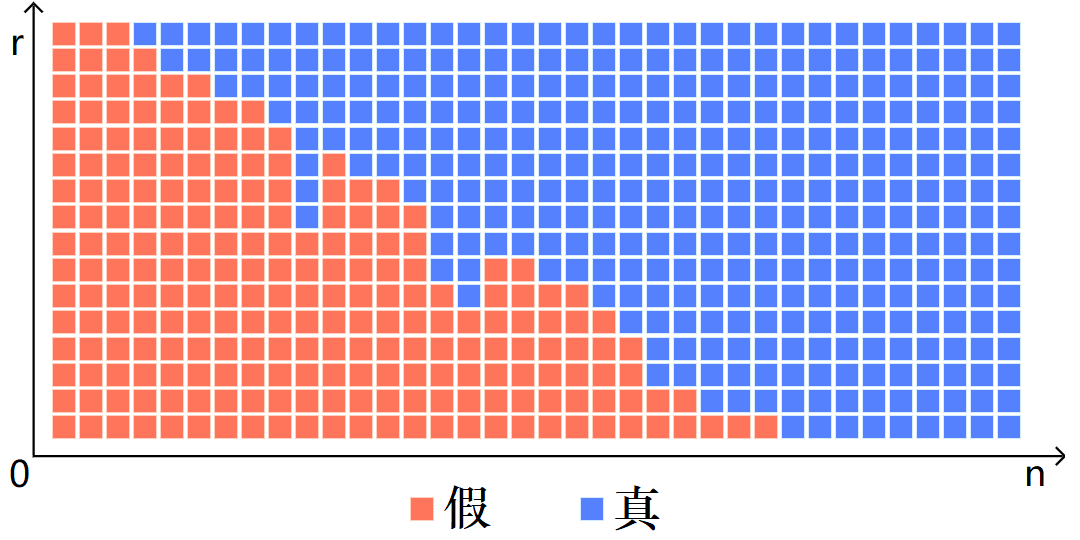
\includegraphics[width=0.64\textwidth]{数列极限2.png}
\end{figure}

每格颜色对应$Q(r, n)$的真假。每一行对应一个正数$r$,每一列对应数列的一个下标$n$。我们的想法是:
不论$r>0$是多少,它对应的行中,$Q(r, n)$必然从某一列起全为真。

我们把$1$称为数列$\{a_n\}$的\textbf{极限}。对一般数列来说,我们定义:
\begin{df}\textbf{数列的极限} \\
设有无穷数列$\{a_n\}$。如果有某个数$x$,使得
$$ \forall r > 0, \,\,\, \exists n,  \,\,\, \mbox{使得} \,\,\, \forall \,\, m \geqslant n, \,\,\, - r \leqslant a_m - x \leqslant r. $$
就说$\{a_n\}$有极限$x$,或$x$是$\{a_n\}$的极限,或$\{a_n\}$趋于$x$,记作
$$\lim_{n\to\infty} a_n = x.$$
\end{df}

\begin{figure}[h] %this figure will be at the right
    \vspace{-14pt}
    \centering
    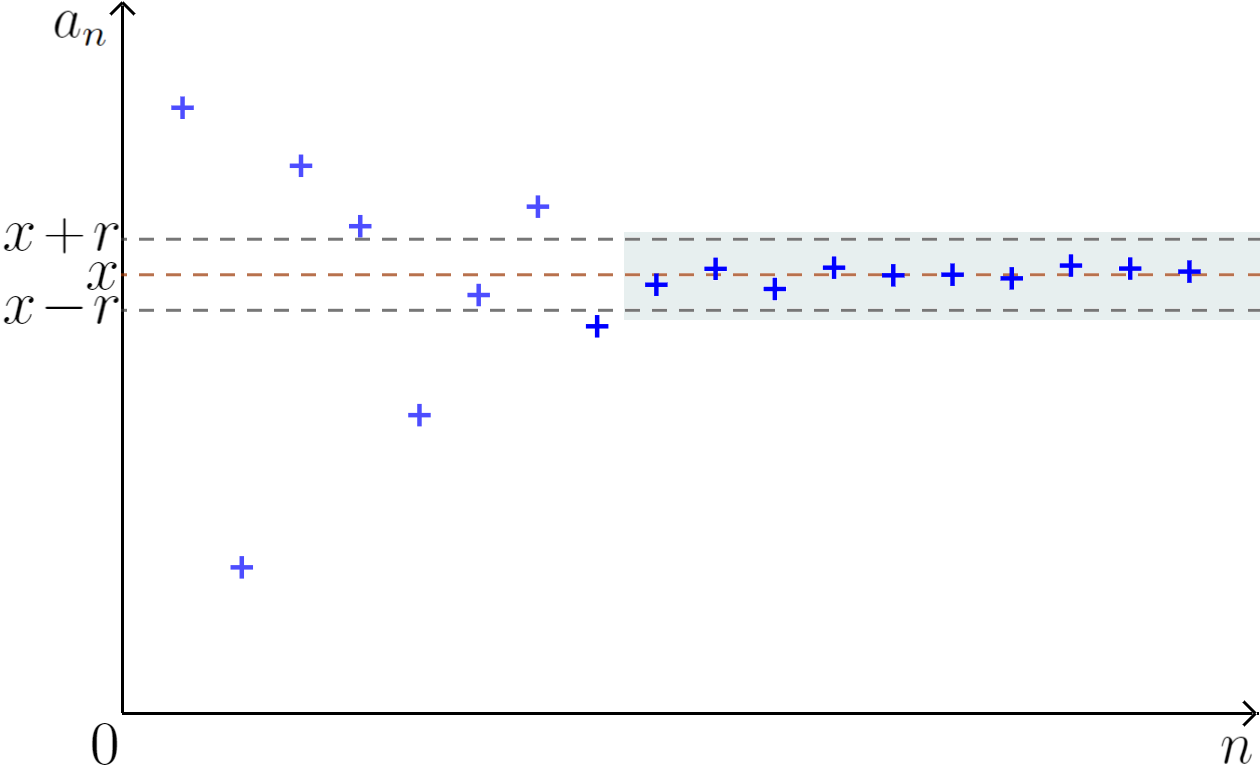
\includegraphics[width=0.54\textwidth]{数列极限1.png}
    \caption*{\texttt{从某一项开始,数列的值总落在区间}$[x-r,x+r]$\texttt{中}}
\end{figure}

\begin{et}
数列$\{a_n\}$的通项是$a_n = \frac{1}{n^2}$,它是否有极限?如果有极限,极限是多少?    
\end{et}
\begin{so}
    $\{a_n\}$每项都是正数。
    $$a_{n} \div a_{n+1} = \frac{1}{n^2} \div \frac{1}{(n+1)^2} = \frac{(n+1)^2}{n^2} = 1 + \frac{2n+1}{n^2} > 1,$$
    所以$\{a_n\}$是单调递减数列。从数轴上看,$\{a_n\}$不断趋近于$0$。猜测它有极限$0$。\\
    设$r>0$,考察区间$[-r,r]$。设$n_r$是大于等于$\frac{1}{\sqrt{r}}$的最小正整数,
    那么,只要$n \geqslant n_r$,就有$n^2 \geqslant n_r^2 \geqslant \frac{1}{r}$,
    于是$0 \leqslant \frac{1}{n^2} \leqslant r$。因此,$\forall r > 0$,$\exists n_r$,
    使得$\forall m \geqslant n_r$,$ -r  \leqslant a_m - 0 \leqslant r$。这说明$\{a_n\}$有极限$0$。    
\end{so}

不难看出,极限是构造出来的。因此,从定义出发,我们可以说某个数是某数列的极限。
反过来,一个数列有极限,它的极限是否只能有一个呢?答案是肯定的。我们可以用反证法来证明。

反设某数列$\{a_n\}$有两个极限$x_1, x_2$。不妨设$x_1 < x_2$。直觉上,$n$足够大的时候,$a_n$在数轴上离$x_1, x_2$都很近,
到两点的距离比$x_2 - x_1$的一半都小,加起来就小于$x_2 - x_1$,于是就产生矛盾了。

具体来说,记$\delta = \frac{x_2 - x_1}{2}$为两点距离的一半。选一个小于$\delta$的正数$r$。
按照极限的定义,有正整数$n_1, n_2$使得:
\begin{align}
    \forall m \geqslant n_1 , \,\,\,& -r \leqslant a_m - x_1 \leqslant r , \notag \\
    \forall m \geqslant n_2 , \,\,\,& -r \leqslant a_m - x_2 \leqslant r . \notag 
\end{align}
于是,选一个比$n_1,n_2$都大的$m$,比如$m=n_1+n_2$,这时$a_m - x_1 \leqslant r$,$x_2 - a_m \leqslant r$。
加起来就得到:
$$x_2 - x_1 \leqslant 2r < 2\delta = x_2 - x_1.$$
矛盾!因此,\textbf{数列如果有极限,只能有一个。}

设数列$\{a_n\}$有极限$x$。我们把它每一项减去$x$(或者说让数列减去常数列$\{x\}$),
得到的数列$\{a_n - x\}$趋于$0$。所以,任何有极限的数列,都可以看做一个趋于$0$的数列加上它的极限。
我们把趋于$0$的数列称为\textbf{无穷小}。任何有极限的数列,都是它的极限加上无穷小。

极限描述了数列的项在“远处”的特征。我们把数列下标超过一定限度后的特征称为数列的\textbf{大体行为}。
有极限的数列,我们可以用极限来刻画数列的大体行为(落在极限“附近”)。
没有极限的数列,大体行为有什么特征呢?

我们来看另一个数列:
$$ 1,\,\,2,\,\,3,\,\,4,\,\,5,\cdots $$
它是正整数数列,通项为$a_n = n$。不难看出,它没有极限。因为对任何实数$x$来说,
令$n_x$为大于$x$的最小正整数,那么从$n_x+1$开始的项都比$x$大至少$1$,
无法落到$x$附近的小区间里面。可以说,随着$n$增大,$a_n$会比任何数都大。

如何严谨描述这个想法呢?我们仍然可以用“有求必应”的结构,把以上想法写成:
$$ \forall x, \,\,\, \exists n, \,\,\,\mbox{使得} \,\,\,\forall \,\, m \geqslant n,,\,\,\, a_m \geqslant x.$$
直观来看,随着$n$增大,从某一项开始,$a_n$会落到数轴任何给定点$x$的右边。
我们把这个性质称为数列\textbf{趋于正无穷大}。同理,可以定义数列\textbf{趋于负无穷大}:
$$\forall x, \,\,\, \exists n, \,\,\,\mbox{使得}\,\,\,\forall \,\, m \geqslant n,,\,\,\, a_m \leqslant x.$$
直观来看,随着$n$增大,从某一项开始,$a_n$会落到数轴任何给定点$x$的左边。

\begin{wrapfigure}[9]{r}{0.33\textwidth} %this figure will be at the right
    \vspace{-48pt}
    \flushright
    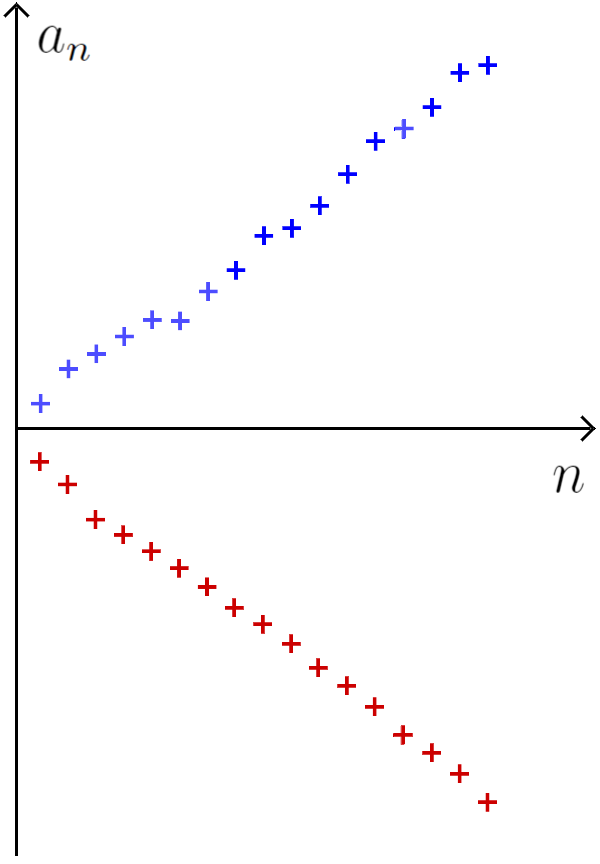
\includegraphics[width=0.32\textwidth]{数列无穷大1.png}
    \caption*{\texttt{趋于无穷大的数列}}
\end{wrapfigure}

我们也把有这两个性质的数列简称为\textbf{正无穷大}和\textbf{负无穷大}。

\begin{et}
    设数列$\{\frac{1}{n}\}$的部分和数列为$\{a_n\}$,证明:$\{a_n\}$趋于正无穷大。
\end{et}
\begin{proof2}
    按照定义,$ a_n = 1 + \frac{1}{2} + \cdots + \frac{1}{n}$。\\
    $a_{n+1} - a_n = \frac{1}{n+1} > 0$,所以$\{a_n\}$单调递增。\\
    对任意实数$x$,我们需要找到相应的$n$,使得$\forall m \geqslant n$,$a_m \geqslant x$。
    由于$\{a_n\}$单调递增,只要某一项$a_n \geqslant x$,它之后的项都大于等于$x$。
    因此,只需要找到$n$使得$a_n \geqslant x$即可。\\
    如果$x \leqslant 1$,那么$n=1$即满足要求。\\
    如果$x > 1$,设$M$是大于$x$的最小整数,考虑$n = 2^{2M}$。下面证明$a_{2^{2M}}>x$。\\
    $$ a_{2^{2M}} = a_{2^0} + \sum_{i=1}^{2M}a_{2^i} - a_{2^{i-1}}.$$
    \begin{align}
        \forall \,\, i\in[1\ldots 2M],\,\,\, a_{2^i} - a_{2^{i-1}} &= \frac{1}{2^{i-1}+1} + \frac{1}{2^{i-1}+2} + \cdots + \frac{1}{2^{i}} \notag \\
        &\geqslant \frac{1}{2^{i}} + \frac{1}{2^{i}} + \cdots + \frac{1}{2^{i}} \notag \\
        &= \frac{2^{i-1}}{2^{i}} = \frac{1}{2}. \notag
    \end{align}
    $$ \mbox{所以}\quad  a_{2^{2M}} \geqslant a_1 + \frac{1}{2} \cdot (2M - 1) = M + \frac{1}{2} > x. $$
    这就证明$\{a_n\}$趋于正无穷大。
\end{proof2}

\begin{sk}
    \mbox{} \\
    \indent 1. 张三在判定数列$\{a_n\}$的极限时写到:数$x$满足:
    $$ \forall r > 0, \,\,\, \exists n,  \,\,\, \mbox{使得} \forall \,\, m > n \,\,\, \mbox{都有} x - r < a_m < x + r. $$
    \indent 因此$\{a_n\}$有极限$x$。他的说法对吗?\\
    \indent 2. 李四在判定数列$\{a_n\}$的极限时写到:数$x$满足:
    $$ \forall r > 0, \,\,\, \exists n,  \,\,\, \mbox{使得} \forall \,\, m > n \,\,\, \mbox{都有} x - 2r \leqslant a_m \leqslant x + 2r. $$
    \indent 因此$\{a_n\}$有极限$x$。他的说法对吗?\\
    \indent 3. 一般数列除了有极限和趋于正负无穷大,还可能有什么大体行为?\\
    \indent 4. 单调数列除了有极限和趋于正负无穷大,还可能有什么大体行为?
\end{sk}

\begin{xt}
    \mbox{} \\
    \indent 1. 以下数列是否有极限?如果有极限,是多少?\\
    \indent\indent 1.1. $\{2^{1-n}\}$ \\
    \indent\indent 1.2. $\{(-1)^{n-1}\frac{n+1}{3n+1}\}$ \\
    \indent\indent 1.3. $\{1 - \frac{1}{n^3+1}\}$ \\
    \indent 2. 以下数列是否趋于无穷大?\\
    \indent\indent 2.1. $\{2^{n}\}$ \\
    \indent\indent 2.2. $\{n^2\}$ \\
    \indent\indent 2.3. $\{\frac{2^n}{n^2}\}$\\
    \indent 3. 如果数列$\{a_n\}$趋于$x$,证明:$\{a_n\}$的任何子列趋于$x$。
\end{xt}

我们已经介绍了数列的运算。数列之间可以做加法、减法、乘法。
如果数列$\{a_n\}$、$\{b_n\}$有极限,它们的和、差、乘积是否有极限?
答案是肯定的,并且符合我们的直觉:
\begin{tm}
    若数列$\{a_n\}$趋于$a$,$\{b_n\}$趋于$b$,则
    \begin{align}
        \lim_{n\to\infty} a_n \pm b_n &= a \pm b, \notag \\
        \lim_{n\to\infty} a_n \cdot b_n &= a \cdot b. \notag 
    \end{align}
\end{tm}
特别地,令$\{b_n\}$是常数列,就得到数乘对极限的影响:若数列$\{a_n\}$趋于$a$,则
$$ \forall \,\, t \in \mathbb{R}, \,\,\,  \lim_{n\to\infty} t \cdot a_n = ta. $$
\begin{proof2}
    \mbox{} \\
    首先证明极限的加法:设数列$\{a_n\}$趋于$a$,$\{b_n\}$趋于$b$。按照定义,$\forall r > 0$,
    由于$\frac{r}{2}>0$,总有正整数$n_a, n_b$,使得
    \begin{align}
        \forall \,\, m \geqslant n_a, \,\,\, & - \frac{r}{2} \leqslant a_m - a \leqslant \frac{r}{2}, \notag \\
        \forall \,\, m \geqslant n_b, \,\,\, & - \frac{r}{2} \leqslant b_m - b \leqslant \frac{r}{2}, \notag 
    \end{align}
    因此,
    \begin{align}
        \forall \,\, m \geqslant n_a + n_b, \,\,\, & -r = - \frac{r}{2} - \frac{r}{2} \leqslant a_m + b_m - a - b \leqslant \frac{r}{2} + \frac{r}{2} = r \notag 
    \end{align}
    于是数列$\{a_n\} + \{b_n\}$趋于$a + b$。\\
    接下来证明极限的数乘:设$t$为实数,数列$\{a_n\}$趋于$a$,则数列$\{t\cdot a_n\}$趋于$ta$。
    这样,数列$\{a_n\} - \{b_n\}$可以看作$\{a_n\} + \{-b_n\}$,因而趋于$a - b$。\\
    分两种情况讨论。如果$t=0$,那么$\{t\cdot a_n\} = \{0\}$,显然趋于$0$,也就是$ta$。
    如果$t \neq 0$,按照定义,对$\forall r > 0$,由于$\frac{r}{t} > 0$,总有正整数$n$使得
    $$ \forall \,\, m \geqslant n, \,\,\, a - \frac{r}{t} \leqslant a_m \leqslant a + \frac{r}{t}. $$
    因此
    $$ \forall \,\, m \geqslant n, \,\,\, ta - r \leqslant t\cdot a_m \leqslant ta + r. $$
    这就说明数列$\{t\cdot a_n\}$趋于$ta$。\\
    最后证明极限的乘法:设数列$\{a_n\}$趋于$a$,$\{b_n\}$趋于$b$。按照定义,$\forall r > 0$,
    由于$\sqrt{r}>0$,总有正整数$n_a, n_b$,使得
    \begin{align}
        \forall \,\, m \geqslant n_a, \,\,\, & - \sqrt{r} \leqslant a_m - a \leqslant \sqrt{r}, \notag \\
        \forall \,\, m \geqslant n_b, \,\,\, & - \sqrt{r} \leqslant b_m - b \leqslant \sqrt{r}, \notag 
    \end{align}
    因此
    \begin{align}
        \forall \,\, m \geqslant n_a + n_b, \,\,\, & (a_m - a)(b_m - b) \leqslant \left(\sqrt{r}\right)^2 = r  \notag \\
        & -(a_m - a)(b_m - b) \leqslant \left(\sqrt{r}\right)^2 = r,  \notag \\
        \mbox{即 }\quad & - r \leqslant (a_m - a)(b_m - b) \leqslant r. \notag 
    \end{align}
    这说明数列$\{(a_n - a)(b_n - b)\}$趋于$0$。而$\{b\cdot a_n\}$和$\{a \cdot b_n\}$都趋于$ab$,
    常数列$\{ab\}$也趋于$ab$,所以根据前面证明的极限加减法,数列
    $$\{a_nb_n\} = \{(a_n - a)(b_n - b)\} + \{b\cdot a_n\} + \{a \cdot b_n\} - \{ab\}$$
    趋于$0 + ab + ab - ab = ab$。
\end{proof2}

四则运算中,加法、减法、乘法都可以对数列的极限做运算。那么除法是否可以呢?
具体来说,若数列$\{a_n\}$趋于$a$,$\{b_n\}$趋于$b$,是否有$\{\frac{a_n}{b_n}\}$趋于$\frac{a}{b}$?

显然,$b=0$的时候,$\frac{a}{b}$无定义,所以排除$\{b_n\}$趋于$0$的情况。如果$b$不等于$0$,
答案大致是肯定的。$\{\frac{a_n}{b_n}\}$趋于$\frac{a}{b}$。
当然,我们要先“剪掉”$\{b_n\}$最开始一些离$b$比较远的项,确保剩下的项都不等于$0$,这样才好定义$\frac{a_n}{b_n}$。
然后可以用类似证明极限乘法的方法,证明$\{\frac{1}{b_n}\}$趋于$\frac{1}{b}$,
这样,$\{\frac{a_n}{b_n}\}$可以看作$\{a_n \cdot \frac{1}{b_n}\}$,因而趋于$\frac{a}{b}$。

\begin{sk}
    \mbox{} \\
    \indent 1. 如果数列$\{a_n\}$有极限$a$,$\{b_n\}$趋于无穷大,它们的和、差、乘积、商数列是否有极限?是否趋于无穷大?\\
    \indent 2. 如果数列$\{a_n\}$、$\{b_n\}$都趋于无穷大,它们的和、差、乘积、商数列有什么特性?
\end{sk}

\begin{xt}
    \mbox{} \\
    \indent 1. 如果数列$\{a_n\}$有极限$a$,$\{b_n\}$趋于无穷大,它们的和、差、乘积、商数列是否有极限?是否趋于无穷大?\\
    \indent 2. 如果数列$\{a_n\}$、$\{b_n\}$都趋于无穷大,它们的和、差、乘积、商数列有什么特性?
\end{xt}

\chapter{从有理数到实数}

\chapter{实变函数初步}

\chapter{二项式}


\end{document}